\documentclass[12pt]{article}
\usepackage{light}

\hidesolutions
%\showsolutions

\newcommand{\edge}[2]{#1\text{---}#2}
\newcommand{\eqdef}{:=}
\newcommand{\suchthat}{\text{ s.t. }}
\newcommand{\rationals}{\mathbb{Q}}
\newcommand{\reals}{\mathbb{R}}
\newcommand{\integers}{\mathbb{Z}}
\newcommand{\naturals}{\mathbb{N}}
\newcommand{\union}{\cup}
\newcommand{\intersect}{\cap}

%\newcommand{\divides}{\mid}
%\newcommand{\ceil}[1]{\left\lceil#1\right\rceil}
%\newcommand{\floor}[1]{\left\lfloor#1\right\rfloor}

\newcommand{\arc}[2]{#1\!\longrightarrow\!#2}

\newcommand{\mfigure}[3]{\bigskip\centerline{\resizebox{#1}{#2}{\includegraphics{#3}}}\bigskip}

\begin{document}

\recitation{11}{October 19, 2016}

%%%%%%%%%%%%%%%%%%%%%%%%%%%%%%%%%%%%%%%%%%%%%%%%%%%%%%%%%%%%%%%%%%%%%%%%%%%%%%%
%\iffalse
\iftrue
\section*{Chains and antichains}
%When items of a poset are tasks that need to be done and the partial order is a precedence constraint, topological sorting provides us with a legal way to execute the tasks sequentially - i.e., without violating precedence constraints. 
%
%But what if we have the ability to execute more than one task at the same time? For example, say tasks are programs, the partial order indicates data dependence, and we have a parallel machine with lots of processors instead of a sequential machine with only one processor. How should we schedule the tasks? For simplicity, we will assume that all tasks take the same amount of time and that all processors are identical.
%
%Assume all tasks take $1$ unit of time and we have an unlimited number of identical processors. Given a poset of tasks, how long does it take to do all of them? For example, in the clothes example that we saw in lecture, how should we schedule the tasks?
%%\mfigure{!}{2in}{getting-dressed}
%
%In the first unit of time we should do all minimal items, so we would put on our left sock, our right sock, our underwear, and our shirt. In the second unit of time, we should put on our pants and our tie. Note that we cannot put on our left or right shoe yet, since we have not yet put on our pants. In the third unit of time we should put on our left shoe, our right shoe, and our belt. Finally, in the last unit of time we can put on our jacket.
%
%The total time to do these tasks is $4$ units. We cannot do any better than $4$ units of time because there is a sequence of $4$ tasks, each needing to be done before the next, of length $4$. Here, for example, we must put on our shirt before our pants, our pants before our belt, and our belt before our jacket. Such a sequence of items is known as a {\it chain}.

Recall some definitions and theorems from lecture. 

\begin{definition} A \term{chain} in a poset $(S, \preceq)$ is a subset $C \subseteq S$ such that for all $x, y \in C$, either $x \preceq y$ or $y \preceq x$.
In other words, it is a sequence $a_1 \preceq a_2 \preceq a_3 \cdots \preceq a_t$, where $a_i \neq a_j$ for all $i \neq j$, such that each item is comparable to the next in the chain, and it is smaller with respect to $\preceq$.
\end{definition}

%
%Thus, the time it takes to schedule tasks, even with multiple processors, is at least the length of the longest chain. Indeed, if we used less time, then two items from the chain would have to be done at the same time, which contradicts the precedence constraints. For this reason, the longest chain is also known as a {\em critical path}. 
%
%Now in this example, we were in fact able to schedule all the tasks in $t$ steps, where $t$ is the length of the longest chain. The really nice thing about posets is that this is always possible! In other words, for any poset, there is a legal parallel schedule that runs in $t$ steps, where $t$ is the length of the longest chain.
%
%There are a lot of ways to prove this fact. Our proof will also give us the corresponding schedule in $t$ time steps, and allow us to obtain some nice corollaries.
%

\begin{theorem}\label{thm:decompose}
Given any finite poset $(A, \preceq)$ for which the longest chain has length $t$, it is possible to partition $A$ into $t$ subsets $A_1, A_2, \ldots, A_t$ such that for all $i \in \{1, 2, \ldots, t\}$ and for all $a \in A_i$, we have that all $b \preceq a$ appear in the set $A_1 \cup \cdots \cup A_{i-1}$. 
\end{theorem}
%Before proving this theorem, first note that for each $i$, all items in $A_i$ can be scheduled in time step $i$. This is because all preceding tasks are scheduled in preceding time steps, and thus are already completed. So the theorem implies that, 
\begin{corollary}
The total amount of parallel time needed to complete the tasks is the same as the length of the longest chain. 
\end{corollary}
%\begin{proof}({\it of Theorem }\ref{thm:decompose})
%For all $a \in A$, put $a$ in $A_i$, where $i$ is the length of the longest chain ending at $a$. We show that for all $i$, for all $a \in A_i$, and for all $b \preceq a$ with $b \neq a$, we have $b \in A_1 \cup A_2 \cup \cdots \cup A_{i-1}$. 
%
%We prove this by contradiction. Assume there is some $i$, $a \in A_i$, and $b \preceq a$ with $b \neq a$ and $b \notin A_1 \cup A_2 \cup \cdots \cup A_{i-1}$. By the way we defined $A_i$, this implies there is a chain of length at least $i$ ending at $b$. Since $b \preceq a$ and $b \neq a$, we can extend this chain to a chain of length at least $i+1$, ending at $a$. But then $a$ could not be in $A_i$. This is a contradiction.
%\end{proof}
%If we have an unlimited number of processors, then the time to complete all tasks is equal to the length of the longest chain of dependent tasks. In recitation you'll see what we can do if there are only a limited number of processors. 
%
%It turns out that the theorem we just proved can be used to do a lot more than schedule tasks for parallel machines. First, we need a definition.
\begin{definition}
An \term{antichain} in a poset $(S, \preceq)$ is a subset $A \subseteq S$ such that for all $x, y \in A$ with $x\ne y$, neither $x \preceq y$ nor $y \preceq x$.). In other words, it is a set of incomparable items, e.g., things that can be scheduled at the same time. 
\end{definition}
%In our clothing example, underwear and shirt form an antichain. Another antichain is left sock, right sock, pants, and ties. 

\section{Problem: Antichains}
The above theorem can be recast in the language of antichains. Prove the following corollary.
\begin{corollary}
If $i$ is the length of the longest chain in a poset $(A, \preceq)$, then $A$ can be partitioned into $t$ antichains.
\end{corollary}
\solution{
\begin{proof}
By the theorem, we can partition $A$ into $t$ sets, where each set consists of tasks that could be scheduled at the same time, i.e., incomparable items. Indeed, if some $x \neq y$ were comparable, then either $x \preceq y$ or $y \preceq x$, and $x$ and $y$ could not be scheduled at the same time.
\end{proof}
}
\emph{Note}: It turns out that the dual of this corollary, which states that if the longest antichain has size $t$, then $A$ can be partitioned into $t$ chains, is also true! However, this is much harder to prove. It is known as \term{Dilworth's theorem}.

%To recap, given any poset, a {\it chain} is a set of distinct items that are all comparable to each other, whereas an {\it antichain} is a set of distinct items none of which are comparable.

\fi

\section{Problem: Taking classes}
Here is prerequistite information for some MIT courses:
%
\begin{align*}
18.01 & \to 6.042 & 18.01 & \to 18.02 \\
18.01 & \to 18.03 & 6.046 & \to 6.840 \\
8.01 & \to 8.02 & 6.01 & \to 6.034 \\
6.042 & \to 6.046 & 18.03, 8.02 & \to 6.02 \\
6.01, 6.02 & \to 6.003 & 6.01, 6.02 & \to 6.004 \\
6.004 & \to 6.033 & 6.033 & \to 6.857
\end{align*}

\begin{enumerate}

\item Draw a Hasse diagram for the corresponding partially-ordered
set.  (Recall: A \term{Hasse diagram} is a way of representing a poset $(A,
\preceq)$ as a directed acyclic graph.  The vertices are the element
of $A$, and there is generally an edge $u \to v$ if $u \preceq v$.
However, self-loops and edges implied by transitivity are omitted.)
You'll need this diagram for all the subsequent problem parts, so be
neat!

\solution[\vspace{0.1in}]{
\ \\
\begin{figure}[h!]
\centering
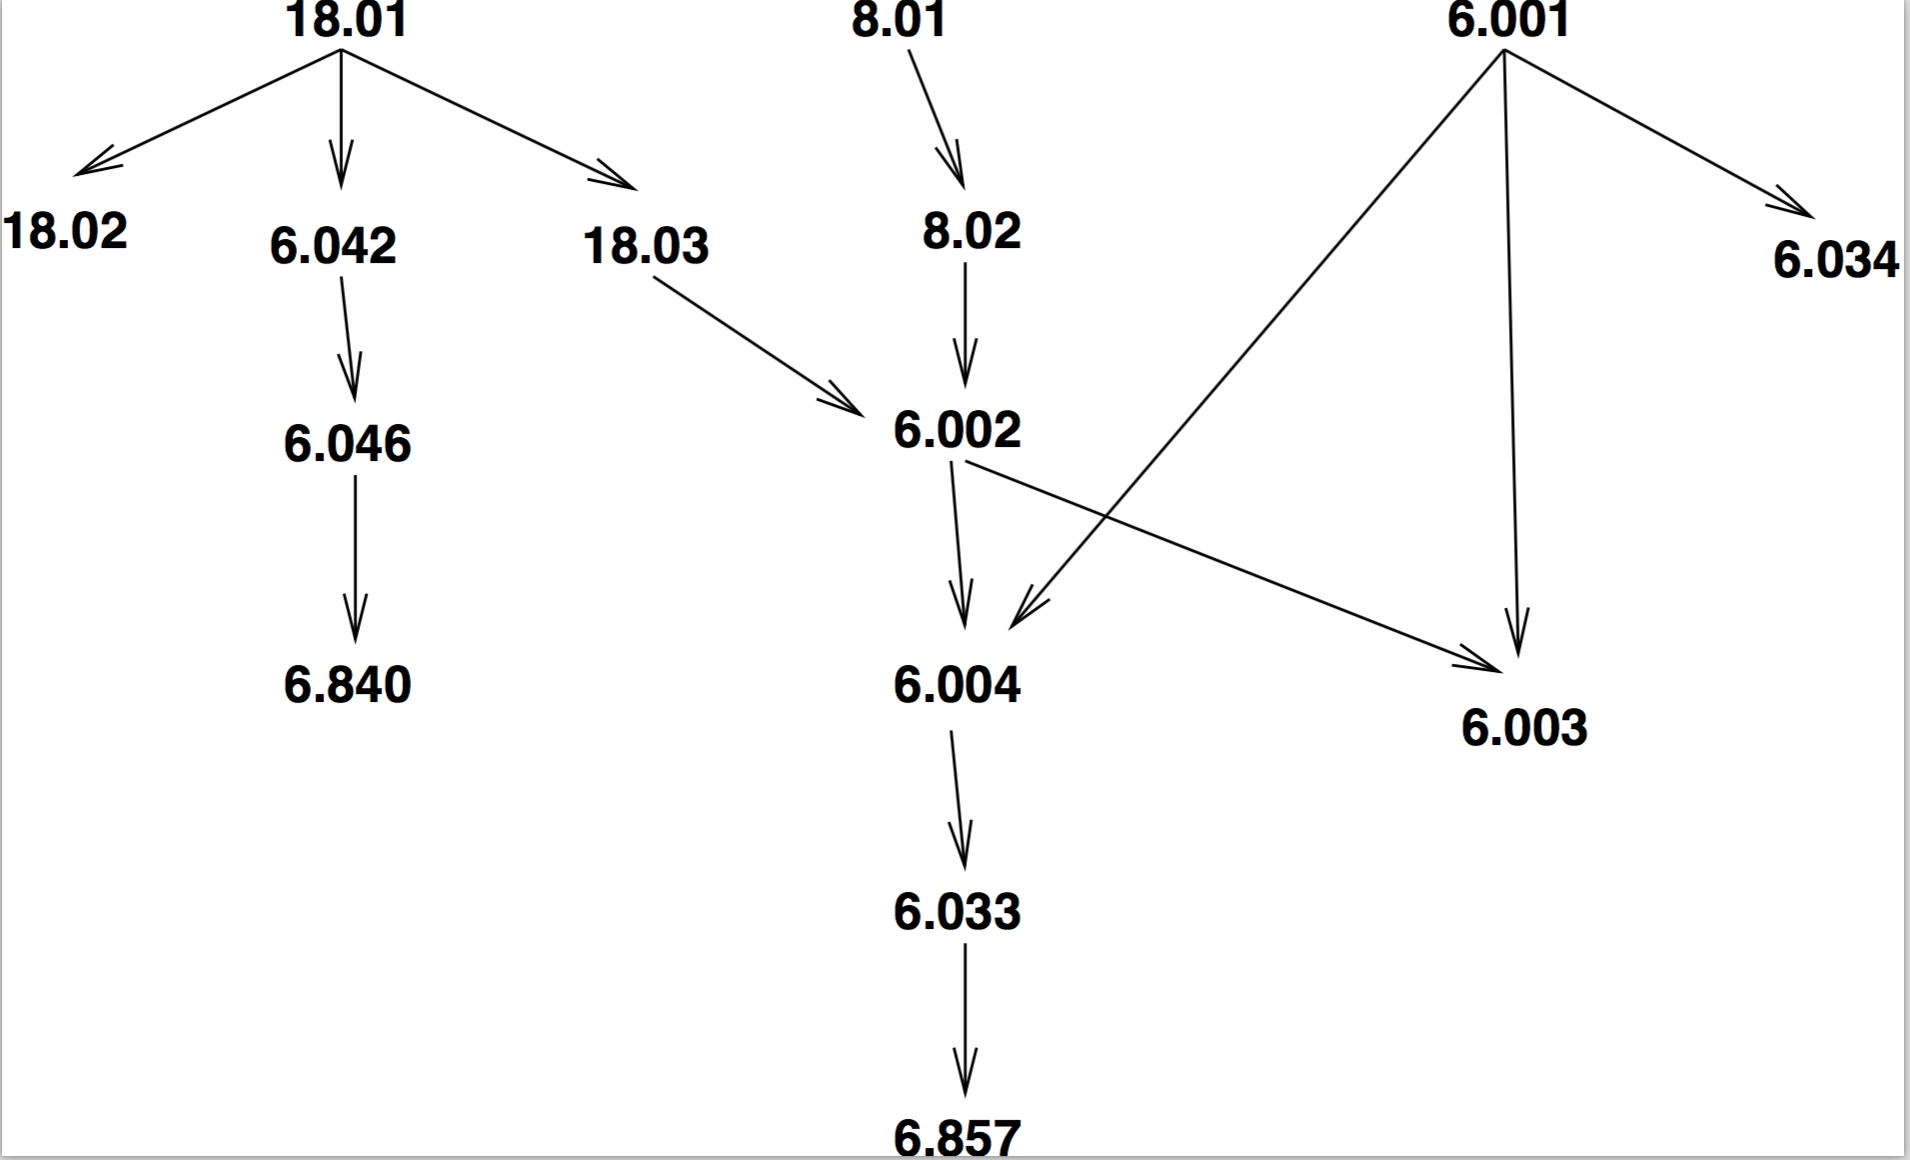
\includegraphics[width=0.8\textwidth]{hasse}
\end{figure}
%\mfigure{!}{2.5in}{rec11-hasse.pdf}
}

\item Identify a largest chain.  %(A \term{chain} in a poset $(S, \preceq)$ is a subset $C \subseteq S$ such that for all $x, y \in C$, either $x \preceq y$ or $y \preceq x$.)

\solution[\vspace{0.1in}]{
There are two largest chains:
\[8.01 \preceq 8.02 \preceq 6.02 \preceq 6.004 \preceq 6.033 \preceq 6.857 \]
\begin{center}and\end{center}
\[18.01 \preceq 18.03 \preceq 6.02 \preceq 6.004 \preceq 6.033 \preceq 6.857 \]
}

\item Suppose that you want to take all the courses.  What is the
minimum number of terms required to graduate, if you can take as many
courses as you want per term?

\solution[\vspace{0.1in}]{Six terms are necessary, because at most one
course in the longest chain can be taken each term.  Six terms are
sufficient by a theorem proved in lecture.}

\item Identify a largest antichain. % (An \term{antichain} in a poset $(S, \preceq)$ is a subset $A \subseteq S$ such that for all $x, y \in A$ with $x\ne y$, neither $x \preceq y$ nor $y \preceq x$.)

\solution[\vspace{0.1in}]{There are several five-element antichains.
One is:
%
\[
\set{18.02, 6.042, 18.03, 8.01, 6.01}
\]
 }

\item What is the maximum number of classes that you could possibly
take at once?

\solution[\vspace{0.1in}]{Classes you are taking simultaneously must
form an antichain, so you can take at most five at once.}

\item Identify a topological sort of the classes.  (A
\term{topological sort} of a poset $(A, \preceq)$ is a total order of
all the elements such that if $a_i \preceq a_j$ in the partial order,
then $a_i$ precedes $a_j$ in the total order.)

\solution[\vspace{0.1in}]{Many answers are possible.  One is 18.01,
8.01, 6.01, 18.02, 6.042, 18.03, 8.02, 6.034, 6.046, 6.02, 6.840,
6.004, 6.003, 6.033, 6.857.}

\item Suppose that you want to take all of the courses, but can
handle only two per term.  How many terms are required to graduate?

\solution[\vspace{0.1in}]{ There are 15 courses, so at least 8 terms
are necessary.  The schedule below shows that 8 terms are sufficient
as well:

\begin{center}
\begin{tabular}{rcc}
1: & 18.01 & 8.01 \\
2: & 6.01 & 18.02 \\
3: & 6.042 & 18.03 \\
4: & 8.02 & 6.034 \\
5: & 6.046 & 6.02 \\
6: & 6.840 & 6.004 \\
7: & 6.003 & 6.033 \\
8: & 6.857
\end{tabular}
\end{center}
}

\item What if you could take three courses per term?

\solution[\vspace{0.1in}]{In part (c) we argued that six terms are
required even if there is no limit on the number of courses per term.
Six terms are also sufficient, as the following schedule shows:

\begin{center}
\begin{tabular}{rccc}
1: & 18.01 & 8.01 & 6.01 \\
2: & 6.042 & 18.03 & 8.02 \\
3: & 18.02 & 6.046 & 6.02 \\
4: & 6.004 & 6.003 & 6.034 \\
5: & 6.840 & 6.033 \\
6: & 6.857 \\
\end{tabular}
\end{center}
}

\item Stanford's computer science department offers $n$ courses,
limits students to at most $k$ classes per term, and has its own
complicated prerequisite structure.  Describe two different lower
bounds on the number of terms required to complete all the courses.
One should be based on your answers to parts (b) and (c) and a second
should be based on your answer to part (g).

\solution[\vspace{0.1in}]{One lower bound is the length of the
longest chain and another is $\lceil n / k \rceil$.}

\item We now complement these lower bounds with an upper bound. This upper bound is known as \term{Brent's Theorem}, and it implies that the \textit{sum} of these two lower bounds is an \textit{upper bound} on the number of terms
required to complete all courses.

Suppose the length of the longest prerequisite chain is $c$. Show that the maximum number of terms required to complete all the courses is 
$$M(n,c,k) \eqdef (c-1) + \ceil{\frac{n-(c-1)}{k}}.$$
\textit{Hint:} Try induction on $c$.  You may find it
helpful to use the fact that if $a\geq b\geq 0$, then
\begin{equation}\label{cab}
\ceil{a-b} \leq 1 + \ceil{a} - \ceil{b}
\end{equation}
for all real numbers $a,b$.

\solution{
Proof by induction.  Induction hypothesis:
\begin{quote}
$P(c) \eqdef \forall \text{ Prerequisite structures }, \forall n,k \in \naturals^+$, if there are $n$ classes with longest prerequisite chain $c$, and if a student can take at most $k$ classes per term,
then the student can take all the classes in $M(n,c,k)$ terms.
\end{quote}

\textbf{Base case $c=1$:} In this case there are $n$ classes and no prerequisites.  So any partition of the classes into $\ceil{n/k}$ blocks
of size at most $k$ will take time
$\ceil{n/k} = 0 + \ceil{(n-0)/k} = M(n,1,k)$.

\textbf{Inductive step:}
Assume $P(c)$ and conclude $P(c+1)$ where $c \geq 1$.

Suppose now that Stanford offers $n$ classes with a longest prerequisite chain size $c+1$.
Suppose $r$ of these classes are endpoints of maximum-size chains.  Note
that none of these $r$ classes can be a prerequisite for another, as otherwise there
would be a chain of length one more than the maximum chain size. Consider the prerequisite schedule obtained by removing these $r$ classes.

Now $H$ is a prerequisite schedule with $n-r$ classes and maximum chain size $c$, so by
the Induction Hypothesis, a student taking at most $k$ classes per term can finish within $M(n-r,c,k)$ terms.

This class schedule can be extended to one for the original prerequisite structure by
arbitrarily grouping $\ceil{r/k}$ of the $r$ classes at endpoints of maximum-size chains, each group of size at most $k$, and taking all classes in a single group in one term. So the total number of terms required is
\begin{align}
\lefteqn{M(n-r,c,k) + \ceil{\frac{r}{k}}}\notag\\
  & = (c-1) + \ceil{\frac{n-r-(c-1)}{k}} + \ceil{\frac{r}{k}} & \text{(def of $M$)}\notag\\
  & = (c-1) + \ceil{\frac{n-c}{k} - \frac{r-1}{k}} + \ceil{\frac{r}{k}}
\label{t1}
\end{align}

We complete the proof by showing that the expression~\eqref{t1} is $\leq
M(n, c+1, k)$.  To do this, we consider two cases:

\begin{itemize}

\item \textbf{Case 1} ($r-1$ is not a multiple of $k$):
We have
\begin{equation}\label{k1}
\ceil{\frac{r-1}{k}} = \ceil{\frac{r}{k}},
\end{equation}
so
\begin{align*}
\text{\eqref{t1}}
   & \leq (c-1) + \left(1+ \ceil{\frac{n-c}{k}} -
   \ceil{\frac{r-1}{k}}\right) + \ceil{\frac{r}{k}} & \text{(by~\eqref{cab})}\\
   & = (c-1) + \left(1+ \ceil{\frac{n-c}{k}} -
      \ceil{\frac{r}{k}}\right) + \ceil{\frac{r}{k}} & \text{(by~\eqref{k1})}\\
   & = c + \ceil{\frac{n-c}{k}}\\
   & = M(n, c+1, k). & \text{(def of $M$)}
\end{align*}

\item \textbf{Case 2} ($r-1$ is a multiple of $k$): 
Now we have
\begin{equation}
\ceil{\frac{r}{k}}=1+\frac{r-1}{k},\label{k+}
\end{equation}
so
\begin{align*}
\text{\eqref{t1}}
  & = (c-1) + \left(\ceil{\frac{n-c}{k}} - \frac{r-1}{k}\right) +
       \ceil{\frac{r}{k}} & \text{(since $(r-1)/k \in \integers$)}\\
  & = (c-1) + \ceil{\frac{n-c}{k}} - \frac{r-1}{k} +
  \left(1+\frac{r-1}{k}\right) & \text{(by~\eqref{k+})}\\
   & = c + \ceil{\frac{n-c}{k}}\\
   & = M(n, c+1, k). & \text{(def of $M$)}
\end{align*}
\end{itemize}
}
\end{enumerate}

%%%%%%%%%%%%%%%%%%%%%%%%%%%%%%%%%%%%%%%%%%%%%%%%%%%%%%%%%%%%%%%%%%%%%%%%%%%%%%%%%%%%%%%%%%%
\section{Problem: Relations}
\begin{enumerate}
\item
Give a description of the equivalence classes associated with each of
the following equivalence relations.

\begin{enumerate}

\item Integers $x$ and $y$ are equivalent if $x \equiv y \pmod{3}$.

\solution[\vspace{0.1in}]{
\[
\begin{array}{l}
\set{\ldots, -6, -3, 0, 3, 6, \ldots } \\
\set{\ldots, -5, -2, 1, 4, 7, \ldots } \\
\set{\ldots, -4, -1, 2, 5, 8, \ldots }
\end{array}
\]}

\item Real numbers $x$ and $y$ are equivalent if $\lceil x \rceil =
\lceil y \rceil$, where $\lceil z \rceil$ denotes the smallest integer
greater than or equal to $z$.

\solution[\vspace{0.1in}]{For each integer $n$, all the real numbers
$r$ such that $n - 1< r \leq n$ form an equivalence class.}

\item Vertices $x$ and $y$ in the graph $G$ are equivalent if there
is a path from $x$ to $y$.

\solution[\vspace{0.1in}]{The vertices in each connected component of
$G$ form an equivalence class.}

\end{enumerate}

%%%%%%%%%%%%%%%%%%%%%%%%%%%%%%%%%%%%%%%%%%%%%%%%%%%%%%%%%%%%%%%%%%%%%%%%%%%%%%%

\item
Show that neither of the following relations is an equivalence
relation by identifying a missing property (reflexivity, symmetry, or
transitivity).

\begin{enumerate}

\item The ``divides'' relation on the positive integers.

\solution[\vspace{0.1in}]{This relation is reflexive (since $a \mid
a$) and transitive (since $a \mid b$ and $b \mid c$ implies $a \mid
c$), but not symmetric (since $3 \mid 6$, but not $6 \mid 3$).}

\item The ``implies'' relation on propositional formulas.

\solution[\vspace{0.1in}]{This relation is reflexive since $p \implies
p$.  It is also transitive, since if $p \implies q$ and $q \implies
r$, then $p \implies r$.  However, it isn't symmetric since, for
example, $\texttt{false} \implies \texttt{true}$, but not
$\texttt{true} \implies \texttt{false}$.}

\item The ``intersects'' relation on nonempty subsets of
$\mathbb{N}$.

\solution[\vspace{0.1in}]{The relation is reflexive, since every
nonempty subset $A$ of $\mathbb{N}$ intersects itself.  The relation
is symmetric, because if $A$ intersects $B$, then $B$ intersects $A$.
However, the relation is not transitive; for example, $\set{1, 2}$
intersects $\set{2, 3}$ and $\set{2, 3}$ intersects $\set{3, 4}$, but
$\set{1, 2}$ does not intersect $\set{3, 4}$.}

\end{enumerate}

\end{enumerate}
%%%%%%%%%%%%%%%%%%%%%%%%%%%%%%%%%%%%%%%%%%%%%%%%%%%%%%%%%%%%%%%%%%%%%%%%%%%%%%%

\end{document}
